\documentclass[
  bibliography=totoc,     % Literatur im Inhaltsverzeichnis
  captions=tableheading,  % Tabellenüberschriften
  titlepage=firstiscover, % Titelseite ist Deckblatt
]{scrartcl}

%irgendetwas mit Tabelen und Figuren anders Nummerieren 
\usepackage{chngcntr}
\usepackage{longtable} 

\usepackage{titling}

%Textdatein einfügen
\usepackage{verbatim}

% Paket float verbessern
\usepackage{scrhack}

% Warnung, falls nochmal kompiliert werden muss
\usepackage[aux]{rerunfilecheck}

% unverzichtbare Mathe-Befehle
\usepackage{amsmath}
% viele Mathe-Symbole
\usepackage{amssymb}
% Erweiterungen für amsmath
\usepackage{mathtools}

% Fonteinstellungen
\usepackage{fontspec}
% Latin Modern Fonts werden automatisch geladen
% Alternativ zum Beispiel:
%\setromanfont{Libertinus Serif}
%\setsansfont{Libertinus Sans}
%\setmonofont{Libertinus Mono}

% Wenn man andere Schriftarten gesetzt hat,
% sollte man das Seiten-Layout neu berechnen lassen
\recalctypearea{}

% deutsche Spracheinstellungen
\usepackage[ngerman]{babel}


\usepackage[
  math-style=ISO,    % ┐
  bold-style=ISO,    % │
  sans-style=italic, % │ ISO-Standard folgen
  nabla=upright,     % │
  partial=upright,   % ┘
  warnings-off={           % ┐
    mathtools-colon,       % │ unnötige Warnungen ausschalten
    mathtools-overbracket, % │
  },                       % ┘
]{unicode-math}

% traditionelle Fonts für Mathematik
\setmathfont{Latin Modern Math}
% Alternativ zum Beispiel:
%\setmathfont{Libertinus Math}

\setmathfont{XITS Math}[range={scr, bfscr}]
\setmathfont{XITS Math}[range={cal, bfcal}, StylisticSet=1]

% Zahlen und Einheiten
\usepackage[
  locale=DE,                   % deutsche Einstellungen
  separate-uncertainty=true,   % immer Unsicherheit mit \pm
  per-mode=symbol-or-fraction, % / in inline math, fraction in display math
]{siunitx}

\DeclareSIUnit{\channel}{Channel}
\DeclareSIUnit{\year}{a}

% chemische Formeln
\usepackage[
  version=4,
  math-greek=default, % ┐ mit unicode-math zusammenarbeiten
  text-greek=default, % ┘
]{mhchem}

% richtige Anführungszeichen
\usepackage[autostyle]{csquotes}

% schöne Brüche im Text
\usepackage{xfrac}

% Standardplatzierung für Floats einstellen
\usepackage{float}
\floatplacement{figure}{htbp}
\floatplacement{table}{htbp}

% Floats innerhalb einer Section halten
\usepackage[
  section, % Floats innerhalb der Section halten
  below,   % unterhalb der Section aber auf der selben Seite ist ok
]{placeins}

% Seite drehen für breite Tabellen: landscape Umgebung
\usepackage{pdflscape}

% Captions schöner machen.
\usepackage[
  labelfont=bf,        % Tabelle x: Abbildung y: ist jetzt fett
  font=small,          % Schrift etwas kleiner als Dokument
  width=0.9\textwidth, % maximale Breite einer Caption schmaler
]{caption}
% subfigure, subtable, subref
\usepackage{subcaption}

% Grafiken können eingebunden werden
\usepackage{graphicx}
\usepackage{wrapfig}

% schöne Tabellen
\usepackage{booktabs}
\usepackage[table]{xcolor}

% Verbesserungen am Schriftbild
\usepackage{microtype}

% Literaturverzeichnis
\usepackage[
  backend=biber,
  sorting=none
]{biblatex}
% Quellendatenbank
\addbibresource{lit.bib}
\addbibresource{programme.bib}

% Hyperlinks im Dokument
\usepackage[
  german,
  unicode,        % Unicode in PDF-Attributen erlauben
  pdfusetitle,    % Titel, Autoren und Datum als PDF-Attribute
  pdfcreator={},  % ┐ PDF-Attribute säubern
  pdfproducer={}, % ┘
]{hyperref}
% erweiterte Bookmarks im PDF
\usepackage{bookmark}

% Trennung von Wörtern mit Strichen
\usepackage[shortcuts]{extdash}

%\setcounter{tocdepth}{3} % + subsubsections



\author{%
  Benedikt Lütke Lanfer \\%
  \href{mailto:benedikt.luetkelanfer@tu-dortmund.de}{benedikt.luetkelanfer@tu-dortmund.de}%
  \and%
  Enno Wellmann \\%
  \href{mailto:enno.wellmann@tu-dortmund.de}{enno.wellmann@tu-dortmund.de}%
}
\publishers{TU Dortmund – Fakultät Physik}


\newcommand*\diff{\mathop{}\!\mathrm{d}}

\NewDocumentCommand \OverfullCenter {+m} {
\noindent\makebox[\linewidth]{#1} }

\usepackage{adjustbox}


% %Tabellen und Figuren Einstellung
% \counterwithout{table}{section}
% \counterwithout{figure}{section}
% \renewcommand{\thetable}{\Roman{table}}
% \renewcommand{\thefigure}{\Roman{figure}}

%Richtiges Einrücken
\setlength{\parindent}{0pt}


\title{V46:\\ Faraday-Effekt an Halbleitern}
\author{Benedikt Lütke Lanfer \and Enno Wellmann}
\date{10. Juni 2024}
\publishers{TU Dortmund – Fakultät Physik}

\begin{document}
\begin{titlingpage}
    \begin{center}
        \begin{Huge}
            \textbf{\thetitle\\}
        \end{Huge}
    \end{center}
    \vspace{4cm}
    
\includegraphics[width=\textwidth]{Bilder/Logo_TU.png} \\
    \vspace{4cm}
    \begin{center}
        \begin{huge}
            \theauthor\\
        \end{huge}
        \vspace{0.5cm}
        \begin{Large}
            benedikt.luetkelanfer@tu-dortmund.de\\
            enno.wellmann@tu-dortmund.de\\
            \vspace{1.4cm}
            Bearbeitet: \today\\
            Durchgeführt: \thedate\\
            TU Dortmund – Fakultät Physik\\
        \end{Large}
    \end{center}
\end{titlingpage}
\tableofcontents
\newpage

\section{Zielsetzung}
In diesem Versuch wird der Effekt der Faraday Rotation verwendet um die
effektive Masse der Leitungselektronen in n-dotierten Galliumarsenid zu messen.

\section{Theorie}
In diesem Versuch scheint eine polarisierte elektromagnetische Welle durch
einen Halbleiter. Dieser Halbleiter wird einem Magnetfeld ausgesetzt was zu
einer Verdrehung der Polarisationsachse führt. Diese Begriffe werden im
folgenden definiert

\subsection{Halbleiter \cite[][Kap. 14]{book:expi3}}
Elektronen in Festkörpern haben anstelle von diskret definierten Zuständen
aufenthaltswahrscheinlichkeiten in der Form von Bändern. Leitende Festkörper
zeichnen sich durch Elektronen im ungebundenen Zustand aus. Isolatoren wiederum
haben eine große Bandlücke zwischen den Gebundenen Elektronen und dem ersten
freien Leitungsband. Diese Bandlücke ist bei Halbleitern in der Größenordnung
von etwa $\qty{1}{\eV}$. Die Bandstruktur von Halbleitern ist auch eine Funktion
des Impuls der Elektronen bzw. deren Wellenvektor $\vec{k}$

\subsection{Effektive Masse \cite[][Kap. 14]{book:expi3}}
Die Effektive Masse ist relevant für die Bewegungsgleichungen der Elektronen im
Leitungsband von Halbleitern sowie der Elektronen löcher im Valenzband. Sie
kann anstelle der Masse eines freien Elektrons verwendet werden. Sie ist
definiert als
\begin{align}
	m^* & = \hbar^2 \cdot \frac{d²E}{d k_i d k_j}
\end{align}

\subsection{Zirkulare Doppelbrechung \cite{man_a}}
\begin{figure}[H]
	\centering
	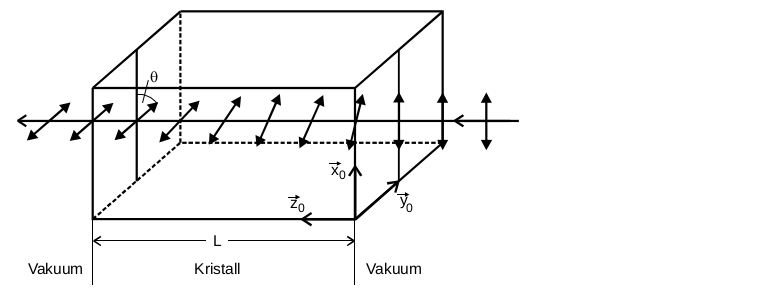
\includegraphics[width=0.8\textwidth]{./Bilder/zirpol.png}
	\caption{Zirkulare Polarisation \cite{man_a} }\label{fig:zirpol}
\end{figure}

Bestimmte Kristalle können die Polarisationsebene eines Linear polarisierten
Lichtstrahls drehen. dies kann dadurch erklärt werden, dass der Brechungsindex
für links und für rechtszirkular Polarisiertes licht unterschiedlich sind. Es
ist möglich das linear polarisierte Licht in eine rechts und eine linkszirkular
polarisierte Welle zu zerlegen.
\begin{align}
	E(z)    & = \frac{1}{2}(E_R(z) + E_L(z))                   \\
	E_R (z) & = (E_0 \vec{x}_0  - i E_0 \vec{y}_0) e^{i k_R z} \\
	E_L (z) & = (E_0 \vec{x}_0  + i E_0 \vec{y}_0) e^{i k_L z} 
\end{align}

Mit den Abkürzungen $ \psi := \frac{L}{2} (k_R + k_L)$ und
\begin{align}
	\theta & := \frac{L}{2} (k_R -k_L)                                    \\
	\intertext{ergibt sich für die Polatisationsebene am Ende des Kristalls mit der Länge $L$}
	E(L)   & = E_0 e^{i\psi} (\cos\theta \vec{x}_0 + sin\theta \vec{y}_0)
\end{align}
Die Phasengeschwindigkeit der Welle kann im allgemeinen durch die relation $V_{Ph}=\omega/k$
ausgedrückt werden. Es folgt
\begin{align}
	\theta &= \frac{L \omega}{2c} \left(\frac{1}{V_{Ph_R}} - \frac{1}{V_{Ph_L}}\right).
	\intertext{Das lässt sich auch bezogen auf die Brechungsindices mit 
	der Vakuumlichtgeschwindigkeit $c$ mit $n = c/v_{Ph}$ darstellen}
	\theta = \frac{L\omega}{2c}(n_R -n_L)
\end{align}


Vielleicht braucht man ja diese Formeln:
\begin{align}
	E                 & = E_L + \frac{\hbar k²}{2 m_e}                 \\
	\frac{d v_g}{d t} & = \frac{1}{\hbar^2}\frac{d^2 E}{d^2 k} \vec{F} \\
	E_e(\vec{k})      & = \frac{\hbar²}{3m^*_e}
\end{align}

\subsection{Fehlerrechnung}
Für die Fehlerrechnung werden alle \textbf{Mittelwerte} von $N$ Messungen
folgendermaßen berechnet:

\begin{equation}
	\overline{x} = \frac{1}{N} \cdot \sum_{i=1}^N x_i
	\label{eqn:Mittelwert}
\end{equation}

und alle \textbf{Standardabweichungen zum Mittelwert} mit:

\begin{equation}
	\increment\overline{x} = \sqrt{\frac{1}{N\cdot(N-1)}\cdot\sum_{i=1}^N (x_i-\overline{x})^2}
	\label{eqn:St_Mittelwert}
\end{equation}

Der Fehler für zusammenhängende Messwerte wird dann mit der \textbf{Gaußschen
	Fehlerfortpflanzung} berechnet:

\begin{equation}
	\increment{f} = \sqrt{ \sum_{i = 1}^{N}  \biggl(\frac{\partial{f}}{\partial{x_i}}\biggr)^2\cdot(\increment{x_i})^2}
	\label{eqn:Gauss}
\end{equation}

Die Fehlerfortpflanzung wird mit Uncertainties in Python \cite{uncertainties}
ermittelt.

%---------------------------------------------------------------------------------------------------------------------------------------------------------------%

\section{Durchführung\cite{man}}% TODO Zahlen überprüfen
Zwei Spulen werden hintereinander mit einem konstanten Strom von
$\qty{10}{\ampere}$ versorgt. Eine Hallsonde wird durch die Spule geschoben um
die Magnetfeldverteilung zu messen. Die Proben werden im Versuch in der
Mitte der Spule eingespannt wo das Magnetfeld am stärksten ist.

Der Versuch wird wie in Abbildung \ref{fig:aufbau} aufgebaut. Weißes licht wird
in einem einstellbaren Polarisator polarisiert und scheint durch die Spule. Im
Zentrum der Spule wird bei dem höchsten Magnetfeld eine Probe mit einer
bekannten Elektronenlochdichte eingespannt. Das Licht fällt danach auf ein
Glen-Thomson Prisma. Es spaltet das Licht in zwei Teile mit zueinander
senkrechter linearer Polarisation. Die beiden Photowiderstände geben ihr Signal
weiter an einen Differenzverstärker. Dessen Signalspannung ist proportional zu
dem Intensitätsunterschied zwischen den beiden Polarisationsachsen. Wenn die
Signalspannung des Differenzverstärkers null (bzw. minimal) wird, ist die
Polarisation genau diagonal zu dem Prisma. Um das Rauschen der Photowiderstände
von dem Lichtsignal zu unterscheiden wird zusätzlich der % Hier die Sorten der Proben einfügen

Der Faraday Effekt rotiert die Polarisationsebene des Lichtes um den Winkel
$\theta$. Das mit einem Goniometer einstellbare Glen-Thomson-Prisma wird auf
den Winkel gedreht, bei dem die Differenzspannung minimal ist.

\begin{figure}
	\centering
	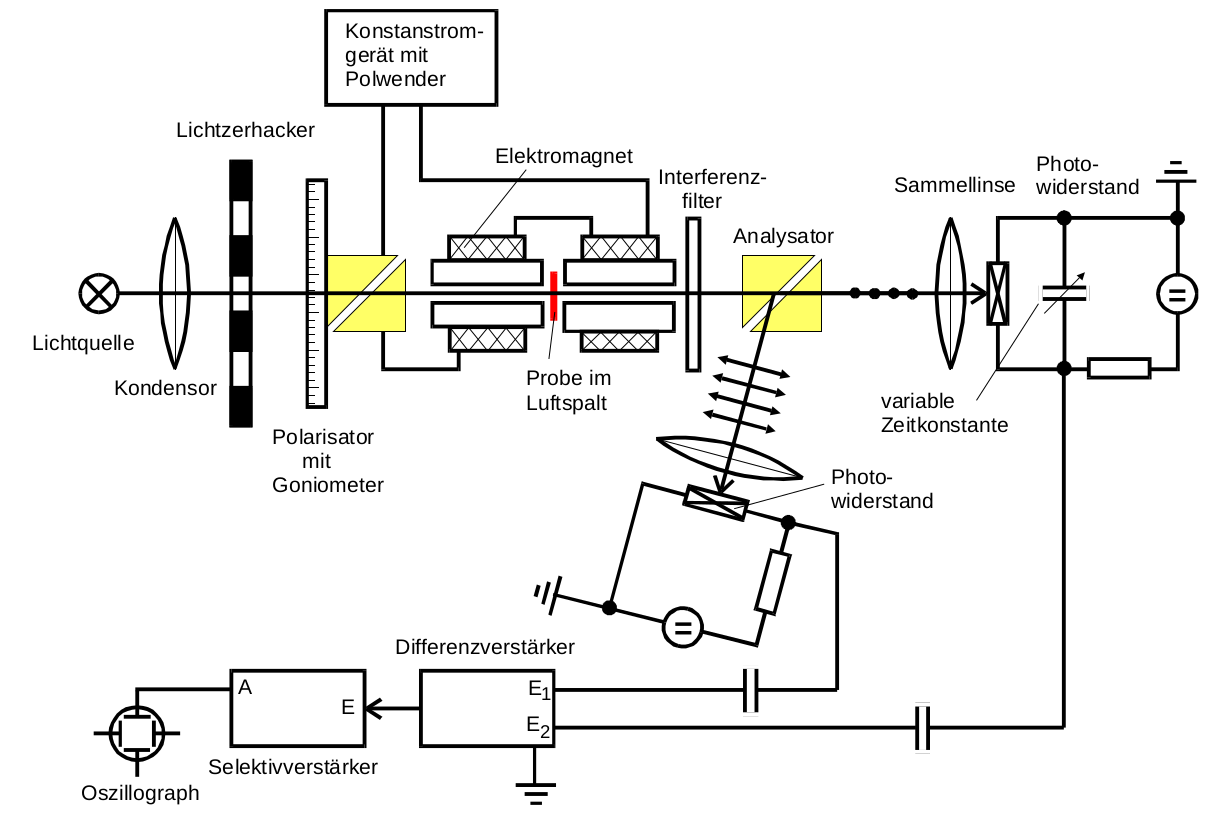
\includegraphics[width=0.8\textwidth]{./Bilder/aufbau.png}
	\caption{Der Versuchsaufbau \cite{man}}\label{fig:aufbau}
\end{figure}




%---------------------------------------------------------------------------------------------------------------------------------------------------------------%

% \section{Durchführung}


%---------------------------------------------------------------------------------------------------------------------------------------------------------------%
\newpage
\section{Auswertung}
\subsection{Bestimmung des B-Feldes}
Die Messung des B-Feldes mittels einer Hall-Sonde ergibt die in Tabelle \eqref{tab:B_Feld} folgende Werte:

\begin{table}[H]
	\centering
	\begin{tabular}{c c}
		\toprule
		$d \, [\unit{\milli\meter}]$ & $B \, [\unit{\milli\tesla}] $  \\
		\midrule
        170 & 1 \\
        160 & 0 \\
        150 & 0 \\
        140 & 0 \\
        130 & 1 \\
        120 & 6 \\
        112 & 92 \\
        110 & 176 \\
        108 & 280 \\
        105 & 382 \\
        102 & 418 \\
        100 & 426 \\
        98  & 428 \\
        95  & 420 \\
        90  & 340 \\
        87  & 236 \\
        85  & 97 \\
        80  & 17 \\
        70  & 0  \\
		\bottomrule
	\end{tabular}
    \label{tab:B_Feld}
\end{table}

Diese Werte werden einmal geplottet \eqref{fig:B_Feld}, welches eine gut sichtbare Parabel förmige Struktur ergibt. 
Jedoch wurden die Werte von $\qty{140}{\milli\meter}$ bis $\qty{170}{\milli\meter}$ ausgelassen das diese Vernachlässigt werden können. 
Das maximale B-Feld ergibt sich dabei mit $B=\qty{428}{\milli\tesla}$ bei $d=\qty{98}{\milli\meter}$. 

\begin{figure}[H]
	\centering
	\includegraphics[width=\textwidth]{build/B_Feld.pdf}
	\caption{Messdaten B-Feld}\label{fig:B_Feld}
\end{figure}

\subsection{Bestimmung der effektiven Masse}
Die Differenz der einzelnen aufgenommen Winkel \eqref{tab:data} je nach B-Feld Ausrichtung werden zuerst mittels 

\begin{equation}
    \Theta =\frac{\theta_2 - \theta_1}{2L} 
\end{equation}

auf die Länge $L$ normiert, welches Faraday-Rotation pro Einheitslänge genannt wird.  
Der Faktor $2$ kommt daher, dass die Differenz des umgepolten B-Feldes doppelt so stark ist wie das vorher bestimmte maximale B-Feld ist. 
Außerdem sind die Messwerte noch in Bogenmaß geben und werden für die folgenden Berechnungen in Radianten umgerechnet. 
Die Proben $1$ und $3$ sind jeweils n-dotiert und die Probe 2 besteht aus reinem $GaAs$. 

\begin{table}[H]
	\centering
	\caption{Messergebnisse der 3 Proben}
	\begin{tabular}{|c|c c c|c c c|c c c|}
		\toprule
		& \multicolumn{3}{|c|}{Probe 1:}  & \multicolumn{3}{|c|}{Probe 2:}  & \multicolumn{3}{|c|}{Probe 3:}   \\
        & \multicolumn{3}{|c|}{$N=\qty[per-mode=fraction]{2.8e18}{\per\cubic\centi\meter} $}  
        & \multicolumn{3}{|c|}{(rein)}  & \multicolumn{3}{|c|}{$N=\qty[per-mode=fraction]{1.28e18}{\per\cubic\centi\meter} $}   \\
        \midrule
        $\lambda \, [\unit{\micro\meter}] $ & $\theta_1$ & $\theta_2 $ &$\Theta_1 [\unit[per-mode=fraction]{\radian\per\meter}]$  
        & $\theta_1 $ & $ \theta_2 $ &$\Theta_2 [\unit[per-mode=fraction]{\radian\per\meter}]$ 
        & $\theta_1 $ & $ \theta_2 $ &$\Theta_3 [\unit[per-mode=fraction]{\radian\per\meter}]$\\
		\midrule
            \num{1.06} & \num{77.50}° & \num{88.60}° & \num{74.74} & \num{70.50}° & \num{93.50}° & \num{39.28} & \num{78.42}° & \num{87.05}° & \num{55.40} \\
            \num{1.29} & \num{78.00}° & \num{86.12}° & \num{54.63} & \num{75.08}° & \num{90.42}° & \num{26.19} & \num{80.17}° & \num{86.93}° & \num{43.42} \\
            \num{1.45} & \num{74.17}° & \num{87.63}° & \num{90.68} & \num{78.50}° & \num{90.50}° & \num{20.49} & \num{80.25}° & \num{88.08}° & \num{50.26} \\
            \num{1.72} & \num{77.08}° & \num{86.48}° & \num{63.30} & \num{78.53}° & \num{87.00}° & \num{14.46} & \num{80.00}° & \num{86.75}° & \num{43.31} \\
            \num{1.96} & \num{71.33}° & \num{87.27}° & \num{107.28}& \num{74.83}° & \num{82.50}° & \num{13.09} & \num{75.33}° & \num{81.08}° & \num{36.90} \\
            \num{2.156}& \num{69.50}° & \num{82.32}° & \num{86.30} & \num{74.67}° & \num{79.17}° & \num{7.68}  & \num{72.78}° & \num{78.83}° & \num{38.82} \\
            \num{2.34} & \num{44.08}° & \num{51.50}° & \num{49.94} & \num{48.50}° & \num{52.50}° & \num{6.83}  & \num{45.25}° & \num{50.25}° & \num{32.08} \\
            \num{2.51} & \num{27.50}° & \num{40.41}° & \num{86.97} & \num{29.17}° & \num{32.33}° & \num{5.41}  & \num{28.25}° & \num{36.00}° & \num{49.73} \\
            \num{2.65} & \num{63.75}° & \num{78.22}° & \num{97.41} & \num{67.83}° & \num{73.17}° & \num{9.11}  & \num{66.60}° & \num{73.08}° & \num{41.60} \\
		\bottomrule
	\end{tabular}
	\label{tab:data}
\end{table}

Diese Faraday Rotation wird im folgenden Plot gegen das Quadrat der Wellenlänge aufgetragen: 

\begin{figure}[H]
	\centering
	\includegraphics[width=\textwidth]{build/Messdaten.pdf}
	\caption{Messdaten Proben}\label{fig:Aufbau}
\end{figure}

Um schließlich die effektive Elektronenmasse zu bestimmen wird jeweils die Differenz zwischen der reinen Probe und den n-dotierten Proben

\begin{align*}
    \Theta_{2,1}&=\Theta_2-\Theta_1  & \Theta_{2,3}=\Theta_2-\Theta_3
\end{align*}

bestimmt.
Schließlich wird diese gegen $\lambda^2$ aufgetragen und mittels der Formel ... jeweils eine Ausgleichsgerade \eqref{fig:plt1} \eqref{fig:plt2} der Form $f(x)=a\cdot x$

\begin{equation}
    \Theta=\underbrace{\frac{NBe_0^3}{8 \pi^2 n \varepsilon_0 c^3} \frac{1}{(m^{\ast})^2}}_{a} \cdot \underbrace{\lambda^2}_{x}
    \label{eqn:theta}
\end{equation}

\begin{figure}[H]
	\centering
	\includegraphics[width=\textwidth]{build/plot2.pdf}
	\caption{Ausgleichsgerade}\label{fig:plt1}
\end{figure}

\begin{figure}[H]
	\centering
	\includegraphics[width=\textwidth]{build/plot1.pdf}
	\caption{Ausgleichsgerade}\label{fig:plt2}
\end{figure}

Die Werte der Ausgleichsgerade 

\begin{align}
    a_{2,1}&=\qty{14.35(1.94)}{\per\cubic\meter} & N&=\qty{2.8e18}{\per\cubic\centi\meter}\\
    a_{2,3}&=\qty{6.24(0.74)}{\per\cubic\meter}  & N&=\qty{1.28e18}{\per\cubic\centi\meter}
\end{align}

sind mittels $curvefit$ von $scipy$ \cite{scipy} bestimmt worden.
Durch Umstellen der Formeln \eqref{eqn:theta} nach der effektiven Masse

\begin{equation}
    m^{\ast}=\sqrt{\frac{NBe_0^3}{8 \pi^2 n \varepsilon_0 c^3} \cdot \frac{1}{a}}
\end{equation}

kann diese schließlich aus den bestimmten Parameter ermittelt werden 

\begin{align}
    \frac{m^{\ast}}{m_0}&=\qty{7.5(0.5)}{\%}\\
    \frac{m^{\ast}}{m_0}&=\qty{7.7(0.5)}{\%}
    \label{eqn:Werte}
\end{align}

welches im Mittel dann $\frac{m^{\ast}}{m_0}=\qty{7.64(0.34)}{\%}$ ergibt

%---------------------------------------------------------------------------------------------------------------------------------------------------------------%

\section{Diskussion}
Aus der Vermessung des B-Feldes lässt sich gut ein maximales B-Feld $B=\qty{428}{\milli\tesla}$ von ablesen. 

Die Messung des Faraday Winkel stellt sich als schwierig und ungenau heraus. 
So ist die Minimierung des Signals durch Verstellen des Winkels ungenau und nicht exakt, 
da durch das starke Schwanken des Signals auf dem Oszilloskop, ein genauer minimaler Winkel nicht auf eine Nachkommastelle einstellbar ist. 
So mit weichen auch die ermittelten Werte \eqref{eqn:Werte}, für die effektive Elektronenmasse, 
im Mittel um $\qty{12.3}{\%}$ von dem Literaturwert von $\frac{m^{\ast}}{m_0}=\qty{6.7}{\%}$ \cite{web:GaAs} ab.


%---------------------------------------------------------------------------------------------------------------------------------------------------------------%
\newpage
\printbibliography

\end{document}